\subsection{Results}

Other methods for calculating local PCQA exist [REF-Leihui], however this is a very time consuming method. Since this method utilize a neural network to predict the surface density/quality the predictions are instant, so the time consuming process of this method lies in the extraction of features. This process is done without looping but for a whole pointcloud in one go and the time it takes is related to how many points exist in the pointcloud. To determine the time taken for feature extraction, a pointcloud was created on the Ball (figure \ref{fig:part_shapes_grid}), but where the ball was varying in size, resulting in different pointcloud sizes. Figure \ref{fig:time} shows the time consumption of extracting features on these pointclouds.

\begin{figure}[htbp]
    \centering
    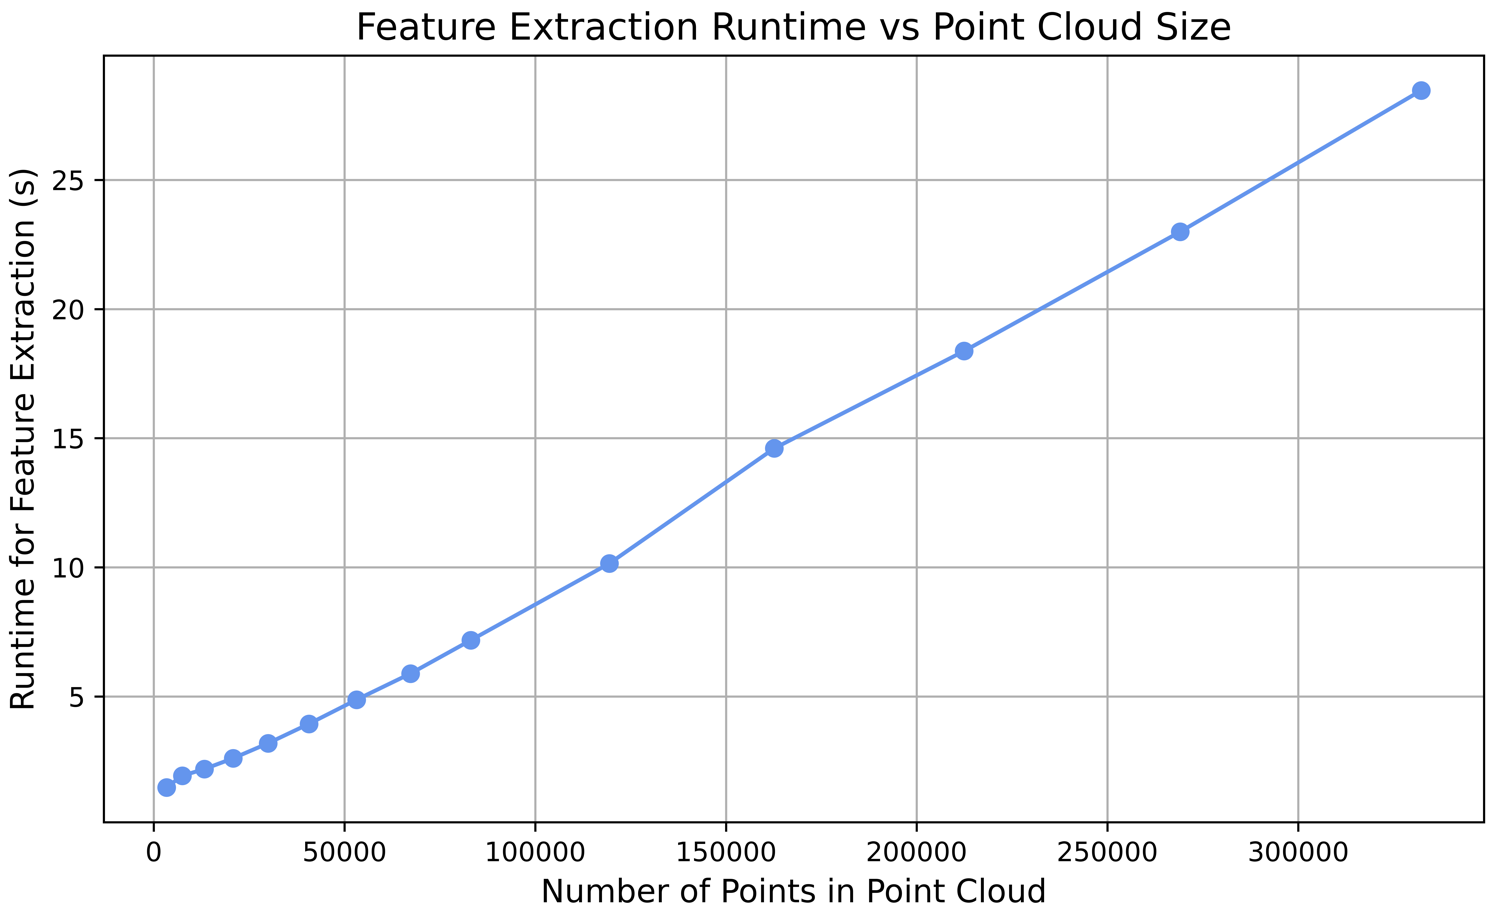
\includegraphics[width=0.5\textwidth]{figures/time_lowQ.png}
    \caption{Feature extraction time consumption for different pointcloud sizes.}
    \label{fig:time}
\end{figure}

To determine the robustness of the models trained on the two datasets, we use a part that the models haven't seen before which is a chain-wheel, see figure \ref{fig:chain_wheel}. This part will used for all result testing in this section.
\begin{figure}[htbp]
    \centering
    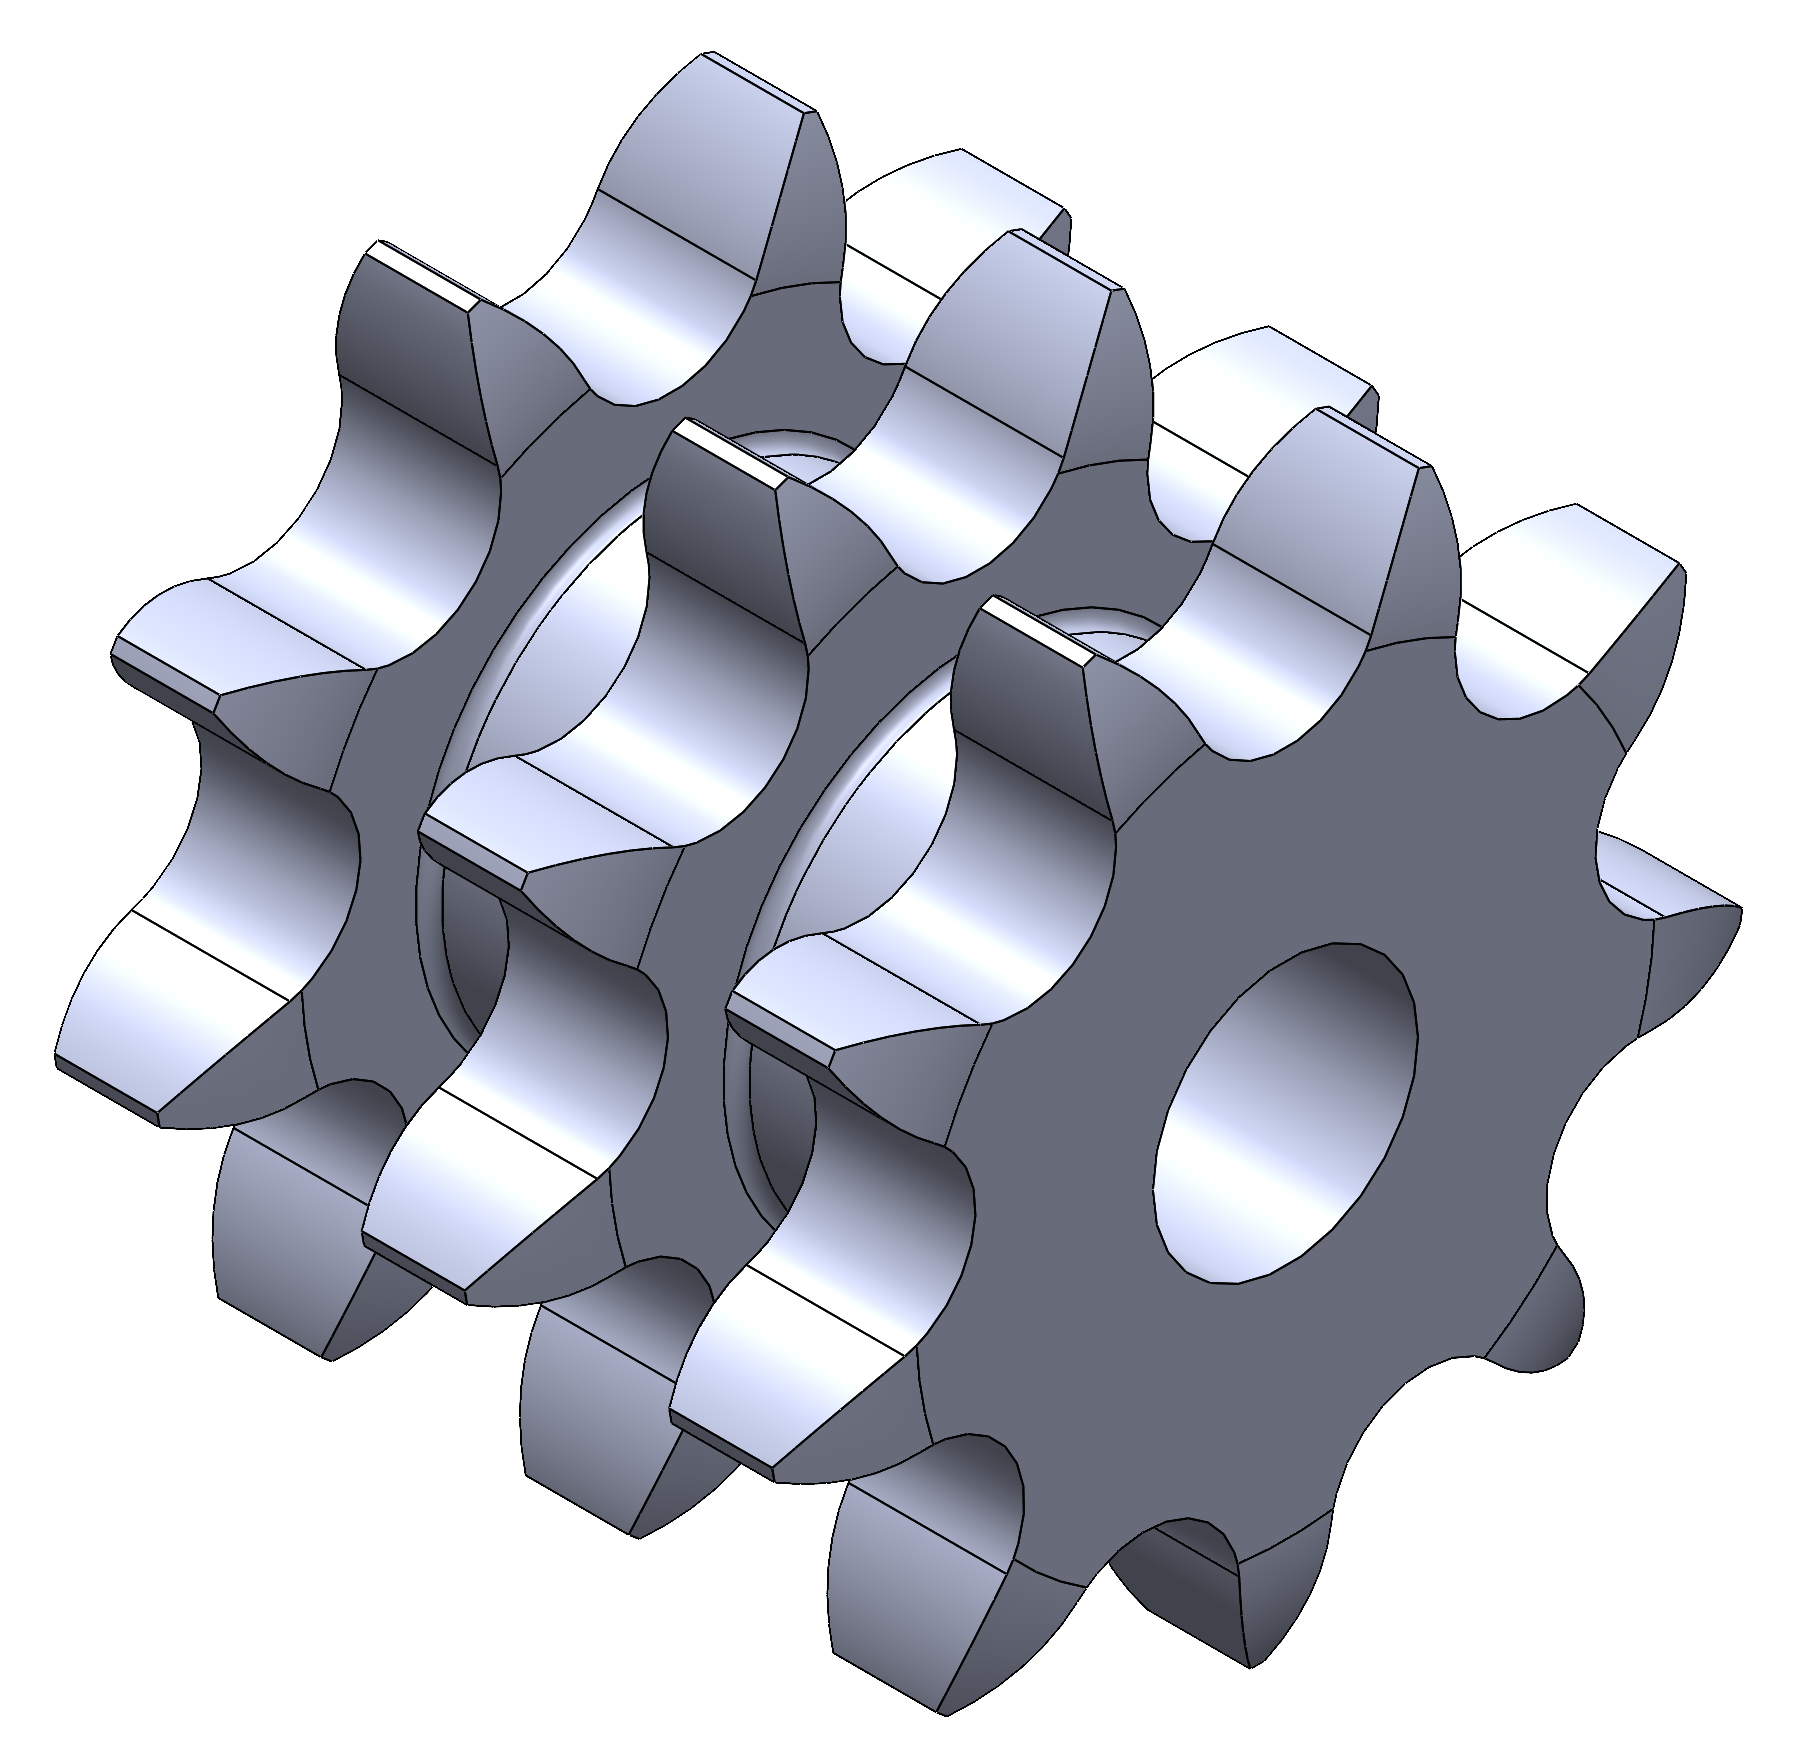
\includegraphics[width=0.3\textwidth]{figures/Chain_whee.PNG}
    \caption{Chain wheel part used for testing the models.} 
    \label{fig:chain_wheel}
\end{figure}

To test the models trained on the two different datasets, the chainwheel was used to generate pointclouds in different mesh sizes to determine the robustness of the models. For the model trained on dataset 1, the predictions are very accurate for a mesh size of 0.5mm and again from meshsizes from 1mm to 2mm. However, mesh sizes between 0.6mm and 1mm gives some wrong predictions so the mean values are much lower than the actual label and the standard deviation is also large, see figure \ref{fig:pred_vs_label_first}.\\
The model trained on dataset 2 is much more robust, showing good predictions for all mesh sizes from 0.5mm to 2mm, with a very low standard deviation, see figure \ref{fig:pred_vs_label_better}. The variation in predictions also follow the tendency of surface density variation for the different mesh sizes as it naturally does as seen in figure \ref{fig:sd_mesh}. Here the variation of surface density is largest at smaller mesh sizes, and decrease as the mesh size goes up.

\begin{figure}[H]
    \centering
    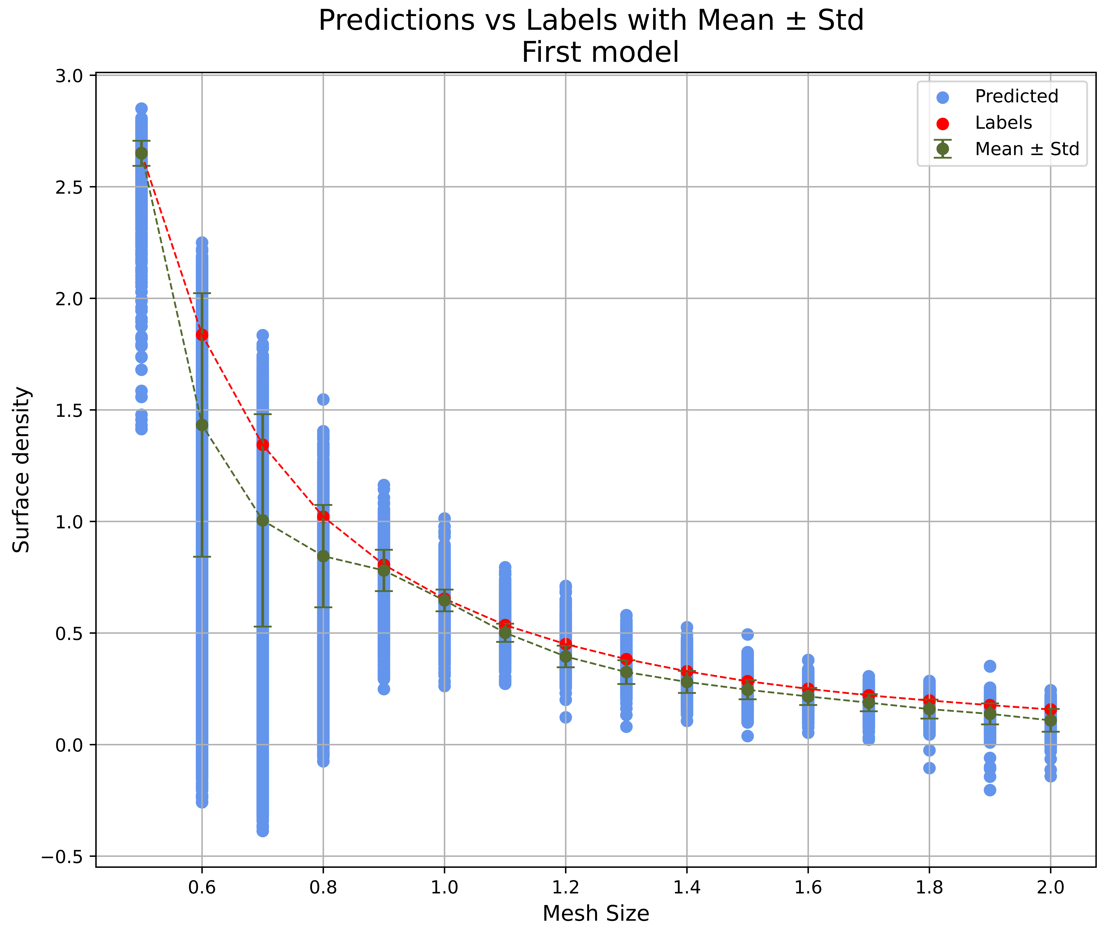
\includegraphics[width=0.5\textwidth]{figures/predict_vs_label_first_lowQ.png}
    \caption{Predicted surface densities vs truth label. Model trained on 0.5, 1.0 and 2.0 mm mesh sizes}
    \label{fig:pred_vs_label_first}
\end{figure}

\begin{figure}[H]
    \centering
    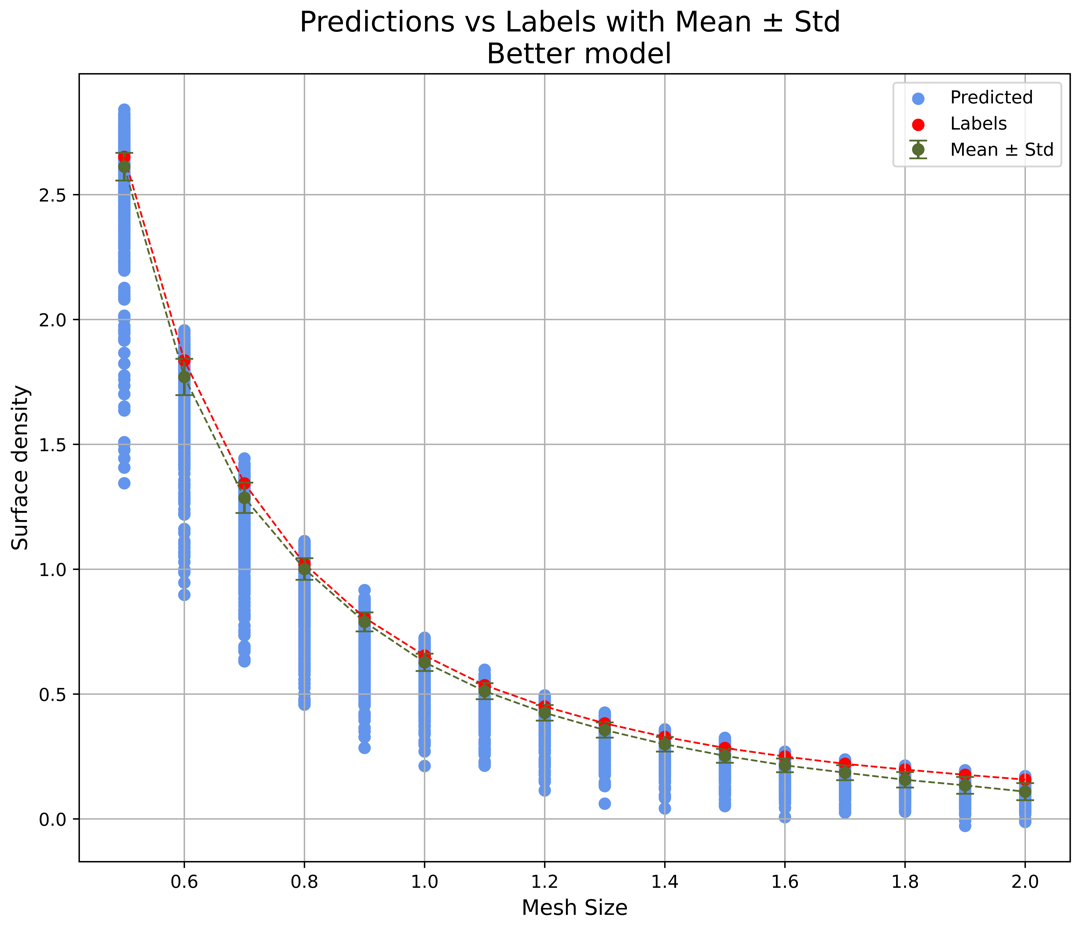
\includegraphics[width=0.5\textwidth]{figures/predict_vs_label_better_lowQ.png}
    \caption{Predicted surface densities vs truth label. Model trained on 0.5 to 2.0 mm mesh sizes with 0.1 mm intervals}
    \label{fig:pred_vs_label_better}
\end{figure}

\begin{figure*}[t]
    \centering
    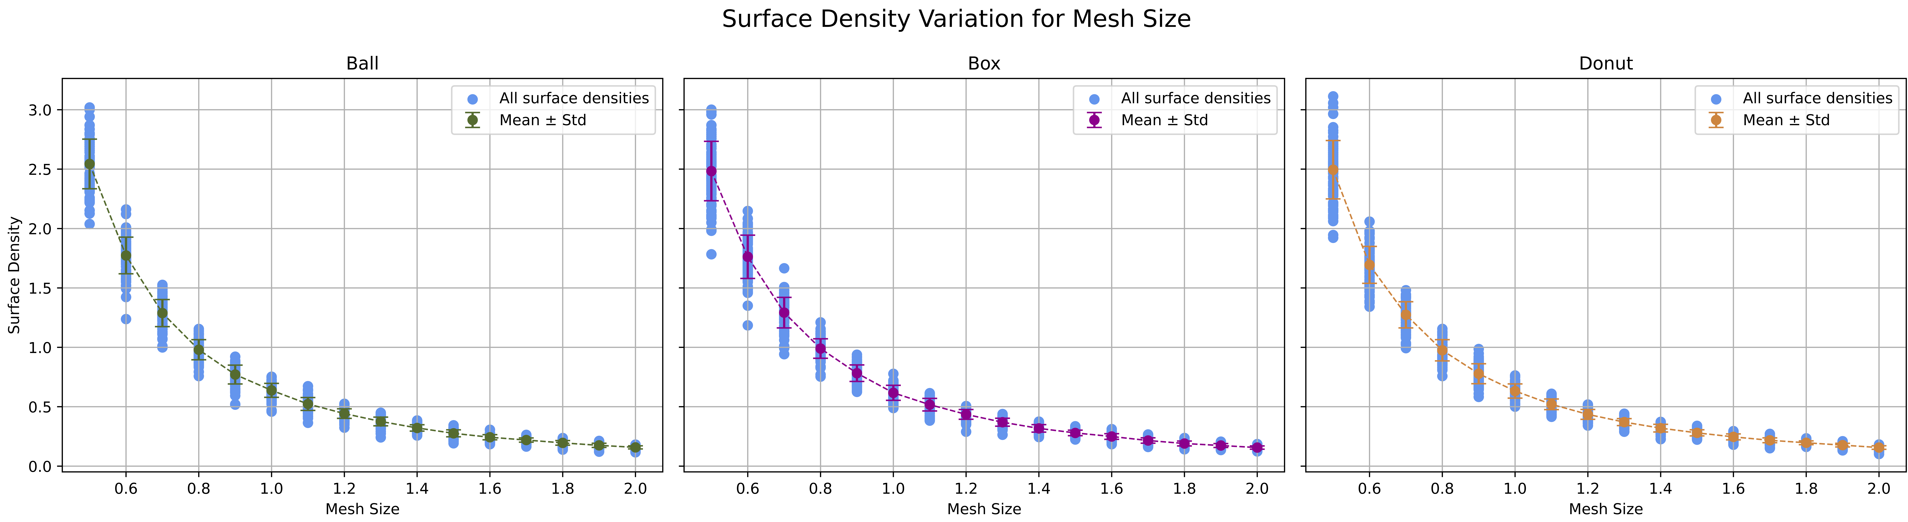
\includegraphics[width=\textwidth]{figures/sd_vs_mesh_lowQ.png}
    \caption{Variation in surface density for different shapes at different mesh sizes}
    \label{fig:sd_mesh}
\end{figure*}

The model should also mark areas where the mesh is incomplete, which simulate missing points that could stem from a incomplete scan of a part. To simulate bad scans holes of different sizes are made in the chain wheel pointcloud and then the quality is predicted. The predictions on these pointclouds shows that the holes are all marked as very low density areas, essentially marking areas where the pointcloud is incomplete, see figure \ref{fig:holes_predict}. The model finds holes as small as 5 points. The model also differentiates between holes that are present in the part and holes that are just from missing points, since the hole that goes through the chain wheel is left as a high density area.

\begin{figure*}[t]
    \centering
    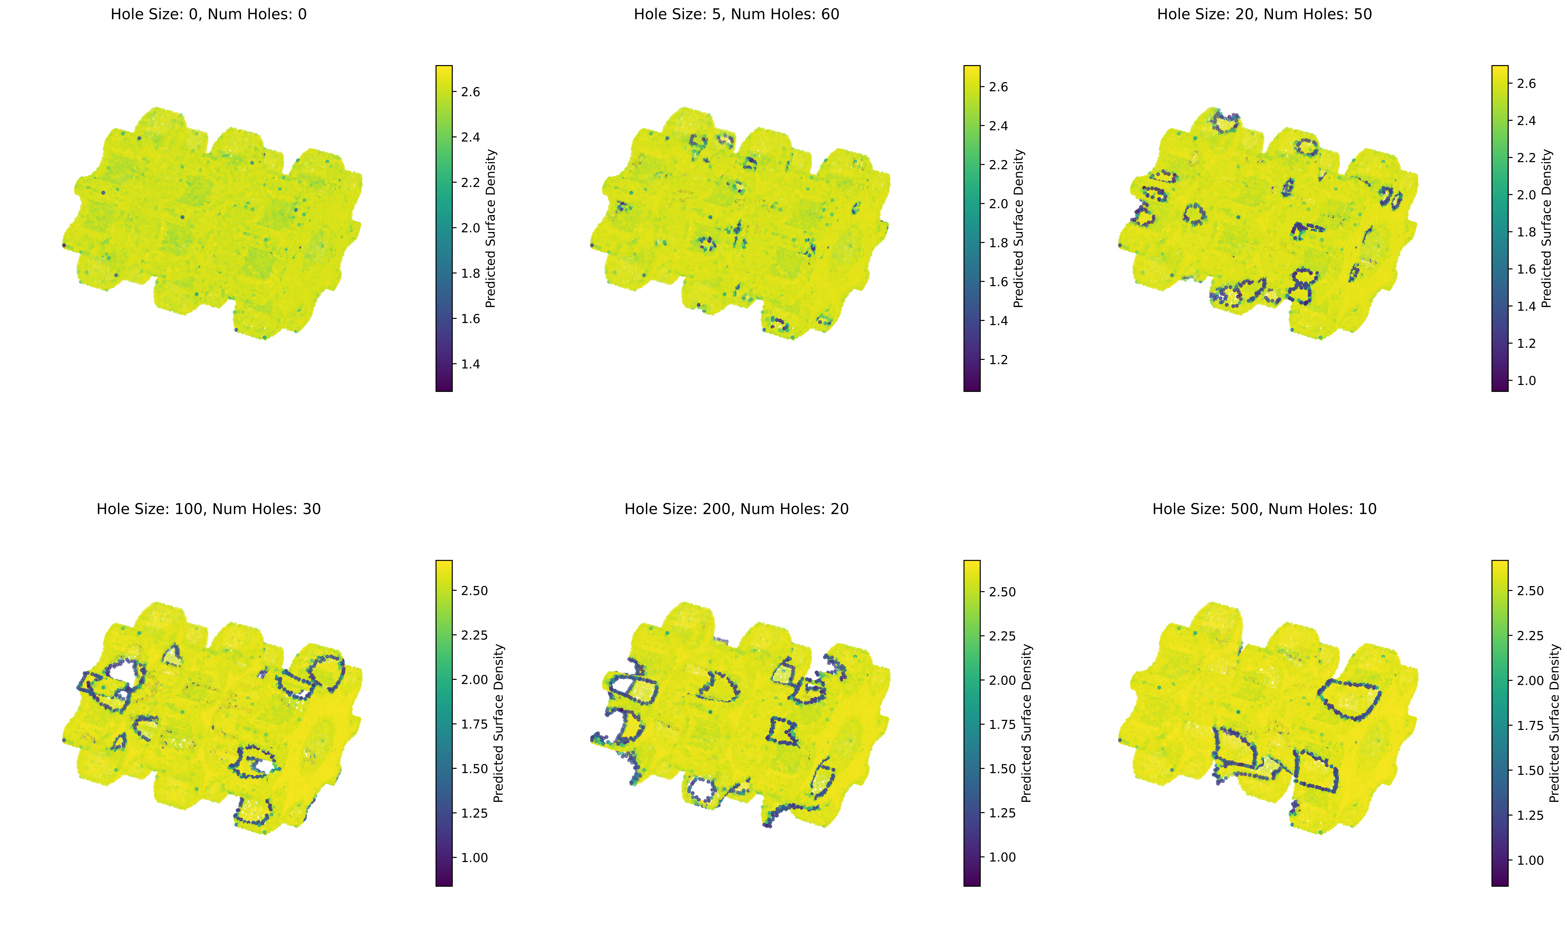
\includegraphics[width=\textwidth]{figures/result3_lowQ.png}
    \caption{Surface density predictions for the same pointcloud with varying hole sizes.}
    \label{fig:holes_predict}
\end{figure*}

The model also excels at predicting the correct surface density on the same part if they vary. This can be seen in figure \ref{fig:diff_mesh_predict}, where the chain-wheel was split up and meshed in different mesh sizes, but the whole pointcloud fed into the model as one pointcloud. Here it is seen that the model is consistent with prediction the correct corresponding surface density.


\begin{figure}[H]
    \centering
    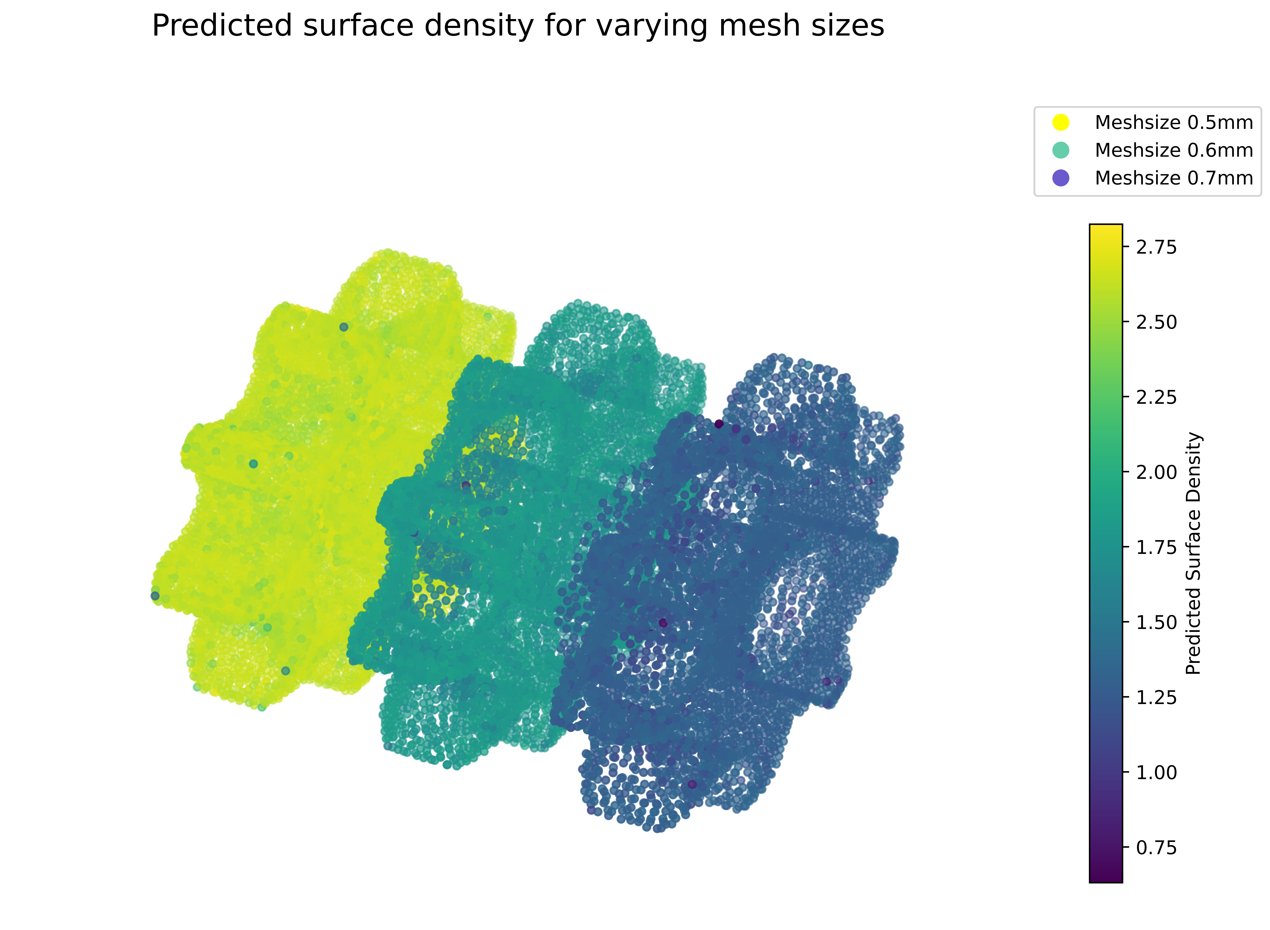
\includegraphics[width=0.5\textwidth]{figures/varying_meshsize_lowQ.png}
    \caption{Surface density predictions for mesh sizes: 0.5, 0.6 and 0.7}
    \label{fig:diff_mesh_predict}
\end{figure}
